\begin{figure*}
    \centering
    % \includegraphics[width=1\linewidth]{images/flowchart.pdf}
    % \includegraphics[width=1\linewidth, height=50mm]{acl-style-files-master-2/images/cacheprune_3.pdf}
    \includegraphics[width=0.87\linewidth, height=48mm]{images/CachePrune_11.pdf}
    % \vspace{-3mm}
    \caption{Illustration of our workflow of CachePrune.
    % defending against indirect prompt injection. 
    Given a prompt with injection, our pruning is guided by a preferential attribution loss computed from sampled clean and poisoned responses.
    Then, we conduct neural attribution using the cached activations from forward-propagation and their gradients from the preferential attribution loss ({\color[rgb]{0.510,0.706,0.882} Blue}). 
    % \textcolor{blue!30}{This is light blue text.}
    % {\color[rgb]{0.510,0.706,0.882} Light blue text}
    % {\color[rgb]{0.510,0.706,0.882} Light blue text}
    During intervention, a neuron is pruned by masking its corresponding row in the context KV cache ({\color[rgb]{0.8,0,0} Red}).
    Activations after step $c_s$ should be generated on the pruned cache. 
    % We use blue arrows for neural attribution and red arrows for pruning.
    % The pruning mask is learnt with only few samples and applied to all the prompts during testing.
    % $\lor$ means the preferential attribution loss is larger when the poisoned response is preferred.
    % over the clean one. 
    % "Forward" and "Gradient" means the neural attribution is computed using the cached activations from forward-propagation and their back-propagated gradients.
    }
    % \vspace{-3mm}
    \label{fig:flow}
\end{figure*}


\section{CachePrune} \label{sec: cacheprune}

\subsection{Preliminary}

\textbf{Prompting LLMs}:
Let $x=[x_t]_{t=1}^T\sim \mathcal X$ denote a prompt with $T$ tokens, consisting of the user instruction and its context as in Figure \ref{fig:demo}.
$p_\theta(\cdot|x)$ is the output probability with an LLM of $L$ layers parameterized by $\theta$. 
% The LLM is expected to answer the user-specified instruction, leveraging the context as data that provides supportive information.
The model is expected to answer the user instruction, while leveraging the context as auxiliary data that provides supporting information.
% Here, the data may not necessarily be numeric, but a text span of supportive information helping address the instruction.

State-of-the-art LLMs generally adopt the Transformer \cite{waswani2017attention} architecture, where each token $x_t$ is encoded by layer $l$ into a key vector $k_{t,l}\in \mathcal R^D$ and a value vector $v_{t,l}\in \mathcal R^D$. 
% $k_t$ and $v_t$ are cached so that they can be reused in response generation. 
Let $\mathcal H_x=[h_t]_{t=1}^T$ be the KV cache of prompt $x$, where $h_t = [k_{t,1}; v_{t,1};\cdots;k_{t,L}; v_{t,L}] \in \mathcal R^{2\times D\times L}$ is the concatenation of key and value vectors from all layers in step $t$.
%that will be reused in response generation. 
% Specifically, let
For a length-$K$ response $y=[y_t]_{t=1}^K\in \mathcal Y$, $y_t$ is generated with,
% %
% \begin{align}
%     p_\theta(y|x) &= \frac{1}{T}\sum_{t=1}^T p_\theta(y_t|x,y_{<t}) \\
%     &= \frac{1}{T}\sum_{t=1}^T p(y_t|\mathcal C, y_{<t}, \theta)
% \end{align}
% %
%
\begin{align}
    p_\theta(y_t|x,y_{<t}) 
    =  p(y_t|\mathcal H_x, y_{<t}, \theta)
\end{align}
%
where $y_{<t}$ denotes the response tokens up to step $t$.  $\mathcal H_x$ is reused during inference with different $y_t$.

\noindent\textbf{Indirect Prompt Injection Attack}:
In an indirect prompt injection attack, there exists additional instructions injected within the prompt context.
% We call an LLM being subjected to prompt injection attack if it is responding to the injected instructions.
As illustrated in Figure \ref{fig:demo}, we define $y^p\sim \mathcal Y^p_x$ as a poisoned response of $x$, if $y^p$ is affected by the injected instructions in the context.
% diverges from the user instruction and follows the injected ones in the context.
Conversely, we define $y^c\sim \mathcal Y^c_x$ as a clean response of $x$, if $y^c$ ignores the injected instructions.
An LLM is considered under attack if $Y^p_x$ is preferred over $Y^c_x$, \emph{i.e.},
%its top response is responding to the injected instructions with g.
%
\begin{equation}
    y^* = argmax_y \,\, p_\theta(y|x) \in  |\mathcal Y^p_x|
\end{equation}
%
$|\cdot|$ is the support of a distribution. 
$y^*$ is approximated with greedy sampling. 
% In greed decoding, An attack happens when the LLM prefers $Y^p_x$ over $Y^c_x$



% Defending against the indirect prompt injection can be viewed as promoting $y_c$ over $y_p$ in the response generation. 
% In this paper, we achieve it by identifying and pruning neurons associated with instruction-following during KV cache encoding of the prompt context.
% by identifying and pruning neurons of the KV Cache that trigger the LLM responding to the injected instructions.
% % in context.
% % We choose to prune on the KV Cache since it is compatible with context caching \cite{gemin_cc, openai_cc}, 
% Importantly, our approach that prunes on the KV Cache is compatible with context caching \cite{gemin-cc, openai-cc}, 
% \emph{e.g.}, enabling efficient prompting when there are multiple questions/instructions with the same cached context.
% For such cases, the KV-Cache of the context or prompts only needs to be pruned once, then reliably saved for future LLM calls without worrying about being attacked by its injections.




\subsection{Defending Against Indirect Prompt Injection Attack} \label{sec: defend}



% % To defend against indirect prompt injection attack, we aim at identifying the difference between  data and instruction from the LLMs' perspective, then enforce such difference between the user-specified context and instruction.
% % Our motivation is to inform the LLM about the boundary between user-specified context and instruction, \emph{i.e.}, the input context should be treated as only pure data.
% % %instead of instructions to follow.

% % To defend against indirect prompt injection attacks,
% % % our approach focuses on distinguishing between data and instructions from the LLM’s perspective, and enforcing this distinction on user-specified context and instructions. 
% % our approach exploits the LLM’s perspective on the distinction between data and instruction, enforcing such distinction between the user-specified context and instructions. 
% % To defend against indirect prompt injection attacks, our approach leverages the LLM’s inherent ability to distinguish between data and instructions,
% % % inforcing this distinction to maintain a clear boundary between user-provided context and instruction.
% % enforcing this distinction over the prompt structure, so the LLM can recognize the boundary between user-provided context and instruction.
% Our approach leverages the LLM’s inherent differentiation between data and instructions. We enforce such distinction over the prompt structure, so the LLM is aware about the boundary between user-provided context and instruction.

% % Our motivation is to ensure that the LLM recognizes the boundary between user-provided context and instructions, by treating the input context strictly as data.
% % We abstract our defense workflow in Figure \ref{fig:flow}.

% % Defending against the indirect prompt injection attack 
% The defending mechanism can be viewed as promoting the clean response $y_c$ over the poisoned response $y_p$. 
% % In this paper, we achieve it by identifying and pruning neurons associated with instruction-following, when encoding KV cache from the prompt context. 
% In this paper, we achieve it by first identifying neurons associated with the LLMs instruction-follow behavior, by learning a pruning mask with \textit{neural attribution}. 
% Then we \textit{intervene} by applying the pruning mask when encoding KV cache from the prompt context. The framework is illustrated in Figure \ref{sec: cacheprune}.

We defend by steering the LLM to interpret the prompt context purely as data rather than as instructions to follow, thereby promoting $Y^c_x$ in response generation.
% Our proposed \textit{CachePrune} is illustrated in Figure \ref{sec: cacheprune}, which is consists of two stages: \textit{Neural Attribution} and \textit{Intervention}.
% Our proposed \textit{CachePrune} consists of an \textit{Neural Attribution} stage and an \textit{Intervention} stage, as illustrated in Figure~\ref{sec: cacheprune}.
To achieve this, we proposed \textit{CachePrune} that defends against the attack in two stages: \textit{Neural Attribution} and \textit{Intervention}, which are illustrated in Figure~\ref{sec: cacheprune}.

% where we first identify neurons associated with the LLMs instruction-follow behavior, by learning a pruning mask with \textit{neural attribution}. 
% Then we \textit{intervene} by applying the pruning mask when encoding KV cache from the prompt context. 

% Our \textit{CachePrune} captures the LLM’s inherent differentiation between data and instructions, by identifying neurons that trigger the LLM’s response to injected instructions.
% We enforcing such differentiation between user-provided context and instruction, so that the context is only interpreted as supportive information instead of any clues for instruction following.
% % over the prompt structure, so the LLM is aware about the boundary between user-provided context and instruction.

% % % As discussed in Section \ref{sec:intro}, an input text span is treated as data if the LLM does not follow its instructions but only leveraging it as supporting information. 
% % Specifically, as discussed in Section \ref{sec:intro}, an input text span is considered data if the LLM leverages it solely as supporting information without following it as an instruction.
% % Therefore, 
% % % the difference between data and instruction is characterized by features in the KV cache that trigger the LLM to follow injected instructions in its response. 
% % we characterize the distinction between data and instruction as features in the prompt KV cache that trigger the LLM to react on injected instructions.
% Specifically, we characterize the LLM's distinction between data and instruction as neurons in the context KV cache that trigger the LLM to react on injected instructions.
% % As defined in \ref{}
% % Such features are identified via features attribution.  and pruned so the input context is treat.
% % We identify such features via \textit{feature attribution}. 
% % Then, we prune such feature on the span of input context, so that the LLM treats the input context as only pure data instead of instructions to follow. 

% The framework is illustrated in Figure \ref{sec: cacheprune}, where we identify these neurons by learning a pruning mask via \textit{neural attribution}, then we \textit{intervene} by applying the learnt pruning mask over the  KV cache of the prompt context.

% We identify these features through \textit{neural attribution} and selectively prune them from the input context span (\emph{i.e., \textit{Context-Aware Pruning}}), ensuring that the LLM interprets the context as pure data.
% % In this way, we enforce the model's awareness on the boundary between input context and instruction.
% %the alignment between the user specified context/instruction and the model's awareness of data/instruction, 
% % This enforcement strengthens the model’s awareness of the boundary between input context and instructions, mitigating the risk of prompt injection attacks.
% % This enforces the LLM's awareness on the boundary between input context and instructions, thus enhancing the model's resilience against prompt injection attacks. 
% The framework is illustrated in Figure \ref{sec: cacheprune}, where we learn a mask on neurons of context KV cache, by attributing from a preferential attribution loss. Below are details of our proposed neural attribution.



\subsubsection{Neural Attribution} \label{sc: na}

% We aim at identifying neurons that contribute to  the LLM-based differentiation on context and instructions.
As mentioned in Section \ref{sec:intro},
we aim at identifying neurons whose
activations bias the LLM’s toward
treating the same context as instructions
to follow rather than as data.
These neurons should not interfere with the model's ability to follow user instructions, \emph{i.e.}, by generating accurate clean responses leveraging the context as data.
The identified neurons are included in a pruning mask derived through the following steps.
% Notable, we regularize with \textit{Selective Thresholding} for the preservation of response quality. 





\vspace{1mm}
% \noindent\textbf{Attribution Scoring.}
% % The goal of feature attribution is to 
% % We aim at identifying key features within the prompt's KV cache that contribute to the observed difference in the LLM's behavior, \emph{i.e.}, when interpreting the input context as either pure data or as instructions.
% % Let $y_c$ and $y_p$ be the poisoned and clean responses give prompt $x$ with injected instructions.
% % Suppose that we have a loss function
% Let $\mathcal L^{attr}: \mathcal Y^c_x\times \mathcal Y^p_x \times\mathcal X \rightarrow \mathcal R$ be an attribution loss function.
% % that captures such difference in LLM outputs.
% Specifically, we have a larger $\mathcal L^{attr}$ indicating the LLM mistakenly treats the input context as instructions, \emph{i.e.}, by preferring a poisoned response $y_p$ over the clean one $y_c$.
% For clarity, we defer the details of the loss function to Section \ref{sec: loss}.


% In attributing $\mathcal L^{attr}$ to neurons in the KV cache,
% we follow \citet{shrikumar2017learning, yang2022task} that score each neuron activation by its contribution to $\mathcal L^{attr}(\mathcal Y^c_x, \mathcal Y^p_x; \mathcal X)$.
% Let $h^i_t$ be the $i$th neuron activation in the key-value vector $h_t$, which is scored by,
% %
% \begin{equation} \label{eq: attr_score}
%     a^i_t = h_t^i \times \pdv{\mathcal L^{attr}(\mathcal Y^c_x, \mathcal Y^p_x; \mathcal X)}{h_t^i}
% \end{equation}
% %
% where $a^i_t$ is the attribution score of $h_t^i$. 
% It is straightforward to see that $h_t^i$ with larger $a^i_t$ suggests a more significant contribution to  $L^{attr}$, thus is more indicative of the model's interpretation on data vs. instruction over the input context.
% % We discuss details of the loss function in Section \ref{sec: loss}.

\noindent\textbf{Attribution Scoring:}
Suppose there exists an attribution loss $\mathcal L^{attr}: \mathcal Y^c_x\times \mathcal Y^p_x \times\mathcal X \rightarrow \mathcal R$
 that captures the model’s preference over which instructions to follow, \emph{i.e.}, by measuring how much it favors a poisoned response over a clean one.
 Neurons contributing more to this loss can be viewed as steering the model to interpret the input as instructions rather than as data.
 % Identifying such neurons therefore reveals the factors underlying this misinterpretation.

 To quantify their contributions, we follow \citet{shrikumar2017learning, yang2022task} and assign an attribution score to each neuron activation based on its influence on $\mathcal L^{attr}$. Let $h_t^i$ denote the activation of the $i$-th neuron at position $t$ in the KV cache. The attribution score $a_t^i$ is defined as:
\begin{equation} \label{eq: attr_score}
a_t^i = h_t^i \cdot \frac{\partial \mathcal{L}^{\text{attr}}}{\partial h_t^i}.
\end{equation}
A larger $a_t^i$ indicates that the neuron activation contributes more to increasing the attribution loss, and is thus more associated with the model’s instruction-following behavior. For conciseness, we defer the details on $\mathcal L^{attr}$ to Section~\ref{sec: loss}.

In our approach, we only score and prune with activations encoded from the text span of input context, as the injected instructions are embedded exclusively within the context.
Let $c_s$ and $c_e$  be the input token index that marks the start and end of prompt context, respectively. 
We denote $\mathcal A=[a_t]_{t=c_s}^{c_e}$ as our attribution matrix and $a_t=[a_t^i]_{i=1}^{2\times D\times L}$ is the attribution vector for $h_t \in \mathcal R^{2\times D\times L}$.
% In the experiments, we compute $\mathcal A$ with $N=8$ samples. $h_{t>{c_e}}$ will be generated with the pruned $\mathcal [h_t]_{t=c_s}^{c_e}$ during testing.


\vspace{1mm}
% \noindent\textbf{Pruning.}
\noindent\textbf{Neural Aggregation:}
% The attribution matrix $\mathcal A$ stores the attribution vector $a_t$ for each $h_t$ from the input context. 
% Note that the features of $\{h_t\}_{t=1}^T$ are not independent on different time steps, but with features on $i$th dimension generated by the same neuron. 
Note that activations of the same neuron share the same dimension $i$ across tokens.
% with the transformer-based language models.
% Accordingly, we aggregate the attribution scores for each neuron by taking its largest value in different time steps,
% Accordingly, we aggregate the attribution scores for each neuron by taking the largest value across time steps,
Thus, we aggregate attribution scores for each neuron by taking the maximum value across the sequence,
%
\begin{equation}
    a^{i,neu} = \max_{c_s\leq t \leq c_e} a^i_t, \,\,\,i\in [1, \cdots, 2\times D\times L]
\end{equation}
%
where $a_i^{neu}$ is the aggregated score of the neuron corresponding to the $i$th dimension.
We take the maximum for each neuron to emphasize its contribution to outputs when the neuron is activated.


% A neuron with large $a^{i,neu}$ is more influential on the LLM's output, \emph{i.e.}, whether treating the context as data or instructions.
% This answers the question raised in Section \ref{sec:intro}: 
% \textit{The activation of such neurons makes a difference on the LLM's view over data vs instruction, by triggering the LLM to respond to the injected instruction in context.} 
% % As mentioned in Section \ref{sec: exp}, our approach is sample efficient, effectively identifying such neurons with only eight samples.


\vspace{1mm}
% \noindent\textbf{Pruning.}
\noindent\textbf{Thresholding:}
% In our approach, we leverage such neurons to enforce the boundary between user-specified context and instruction.
% In our approach, we leverage the identified neurons with large $a^{i,neu}$  to enforce the boundary between user-specified context and instruction.
% % , ensuring that the context is interpreted solely as data by the LLM. 
% On way to achieve this is to prune the top p$\%$ of neurons with the largest value of $a^{i,neu}$ within the prompt context.
% , by setting their corresponding features to zero over the KV cache of input context.
% , \emph{i.e.}, setting their corresponding features to zero.
% By intervening on the activation values of neurons with large $a^{i,neu}$, we should be able to affect the LLM's decision on data vs. instruction.
% Intervening on neurons with large $a^{i,neu}$ should alter the LLM’s interpretation between data and instruction.
Pruning on neurons with large $a^{i,neu}$ should alter the LLM’s tendency of interpreting the context as instructions.
% However, this would result in responses with low quality since our $\mathcal L^{attr}$ is only about poison vs. clean, without considering the response quality.
However, this would degrade the clean responses since our $\mathcal L^{attr}$ only captures the preference over which instructions to follow, 
% without explicitly preserving the role of the context as supporting information for a clean response.
% without regularization on preserving the quality of context as supportive information once the model choose the clean one.
without regularization on preserving the quality of context as supporting information when producing clean responses.
For example, the model may be missing context if pruning disrupts the semantics content.

% Neurons with large $a^{i,neu}$ corresponds to the model's interpretation between data and instruction. 
% However, they may also corresponds to the


To maintain the quality of clean responses after pruning, 
% we only intervene on a subset of neurons $\Phi$ up to p$\%$ of all the neurons.
we regularize by selectively pruning from only a subset $\Phi$ of neuron that excludes those interfering with response quality. The definition of $\Phi$ is introduced in Section \ref{sec: loss}.
We prune from $\Phi$ up to p$\%$ of all the neurons.
% This pruning can be understood as a masking of neuron activations across the span of input context. 
% This pruning can be understood as a masking over the feature dimensions. 
% Such masking is a reflection of the LLM's own identification of what distinguishes pure data from instructions, which is enforced over the context span so that the injected instructions are not responded.
% This pruning effectively acts as a mask over the feature dimensions.
% , reflecting the LLM's own recognition of what differentiates pure data from instructions. 
% As mentioned above, we include the identified neurons for intervention within a pruning mask.
% As mentioned before, the identified neurons are included in a pruning mask for intervention.
Formally, let $\tau$ denote the thresholding value on  $a^{i,neu}$ for the pruning mask,
% %
% \begin{equation} \label{eq: tao}
%     \tau = \text{inf}_{\tau\in\mathbb R} Pr(i|a^{i,neu}\geq \tau, i
%     \in\Phi)\,\,\ \leq \,\, p
% \end{equation}
% %
%
\begin{equation} \label{eq: tao}
    \tau = \text{inf}_{\tau_0\in\mathbb R} \, \mathbb E_i\, ( \mathbbm 1\{a^{i,neu}\geq\tau_0, i\in\Phi\} )\ \leq \,\, p
\end{equation}
%
% $Pr$ is uniform over all neurons. 
where $ \mathbbm 1$ is the indicator function. For the $i$th neuron, its masking value is $\mathbbm 1\{a^{i,neu}\geq\tau, i\in\Phi\} )$.
% The definition of $\Phi$ is explained in Section \ref{sec: loss}, since it depends on $\mathcal L^{attr}$.
% To ensure that pruning does not compromise the quality of the generated clean responses, the $p\%$ neurons are selected from from a set $\Phi$ that will be defined in Section \ref{sec: loss}. 

% Neurons with large $a^{i,neu}$ corresponds to the model's interpretation between data and instructions. 


% We select neurons for pruning via thresholding on  $a^{i,neu}$, selecting neurons with large $a^{i,neu}$ from a set $\Phi$ up to p$\%$ of all the neurons.
% Formally, let $\tau$ denote the thresholding value on  $a^{i,neu}$ for the pruning mask,


\subsubsection{Intervention}

In experiments, the pruning mask is learnt from neural attribution with only few samples, then applied to all the prompt context during testing.
Specifically, 
% we enforce the boundary between the user-defined context and instructions by applying the pruning mask over the prompt context.
% Specifically, for each dimension $i$ in $h_t$, $t\in[c_e,c_s]$, we mask on it by multiplying with $m_i$,
for each $h_t^i$ from the context KV cache with $t\in[c_e,c_s]$, we apply the masking by multiplying with $m_i$,
%
\begin{equation} \label{eq: mask}
    m_i = 1 - \alpha\cdot \mathbbm 1\{a^{i,neu}\geq\tau, i\in\Phi\}
\end{equation}
%

% By enforcing this masking over the context, we ensure that the context is interpreted solely as data by the LLM.
\noindent where $\alpha$ denotes the strength of intervention which defaults to 1. 
In Table \ref{tb:mask}, varying $\alpha$ shows a trade-off between robutness and quality of following user instructions.
$m_i$ reflects the LLM's implicit criteria of what differentiates instructions from data. 
Applying this mask over the prompt context ensures that the model's implicit criteria \textit{aligns} with the 
% user-defined separation between data and instructions as mentioned in Section \ref{sec:intro}.
data-instruction separation specified in the prompt.
% user-defined data-instruction separation as mentioned in Section \ref{sec:intro}.
% the LLM interprete the context solely as data, thus mitigating indirect prompt injection attack.
% $h_{t>{c_e}}$ will be generated with the pruned $\mathcal [h_t]_{t=c_s}^{c_e}$ during testing.
% As mentioned earlier, 
% We abstract our workflow in Figure \ref{fig:flow}.




% \subsection{The Preferential Attribution Loss} \label{sec: loss}
\subsection{The Preferential Attribution Loss} \label{sec: loss}

% According to Section \ref{sec: defend}, the neural attribution is guided by an attribution loss $\mathcal L^{attr}$,
% which quantifies how a poisoned response is favored over a clean one.
% % the observed difference between interpreting the context as either pure data or instructions. 
% % Specifically, the lossis higher when the LLM prefers poisoned responses $\mathcal Y^p_x$ over  $\mathcal Y^c_x$, vise versa.
% This can be evaluated as an objective of preference optimization, among which the most common and effective one is the Direct Preference Optimization (DPO) \cite{rafailov2024direct}.

As described in Section~\ref{sec: defend}, neural attribution is guided by an attribution loss $\mathcal L^{attr}$, which measures how much a poisoned response is favored over a clean one. 
This can be framed as a preferential optimization objective, with Direct Preference Optimization (DPO) \cite{rafailov2024direct} being a widely used and effective example.
In the context of indirect prompt injection, the DPO objective $\mathcal L_{DPO}$ can be defined as,
% \vspace{-2mm}
%
\begin{equation}
  \begin{split} \label{eq:L_dpo_}
    \!\! \mathcal L_{DPO} = &\mathbb  E_{(x,y^c,y^p)\sim \mathcal D} [ \log \,\sigma( \beta\log \frac{p_{\theta}(y^p|x)}{p_{ref}(y^p|x)} \\
    &-\beta\log \frac{p_{\theta}(y^c|x)}{p_{ref}(y^c|x)})].
  \end{split}
\end{equation}
%
where $\beta>0$, $\mathcal D=\{\mathcal X, \mathcal Y^c_x, \mathcal Y^p_x\}$ is the perference optimization dataset and $p_{ref}$ is a reference model. $\sigma(\cdot)$ is the sigmoid function.
% and is a regularization parameter. 
% The reference model $ref$ serves as an anchor that is chosen before training. Specifically, the minimization of $\mathcal L_{DPO}$ is also minimizing the following KL divergence,
% %
% \begin{equation} \label{eq:DPO_KL_}
%     \mathcal D_{KL} [p_{\theta}(y|x)\,||\,p_{ref}(y|x)].
% \end{equation}
% %
% An accurate estimation of $\mathcal L_{DPO}$ will ideally capture the difference between the LLM's interpretation on data vs. instruction. 
% Specifically, 
A higher $\mathcal L_{DPO}$ indicates the context being mistakenly perceived as instruction, and vice-versa.

% \eqref{eq:L_dpo_} has been proven effective when being optimized with a sufficiently large preference dataset with scaled training. 
% For example,  \cite{chen2024aligning} optimize \eqref{eq:L_dpo_} with manually designed preference datasets of clean and poisoned responses. %The resulting model will generally be robust to indirect prompt injection attack.
% However, there is not guaranteed that \eqref{eq:L_dpo_} still induces the optimal results when leveraged for feature attribution to guide the neuron pruning. 
% Actually, though our pruning with feature attribution can be thought of a single-step projected gradient descent on the attribution loss, pruning with feature attribution is not exactly the same as optimization. 
% The former aims at finding the appropriate allocation of contribution to outputs so to rank the importance of each activation, while the later wants to find an reliable direction between updates.
Our attribution loss is a practical simplification from \eqref{eq:L_dpo_}. Let $y^{p,*}_x$ and $y^{c,*}_x$ be the most probable poisoned and clean responses from prompt $x$. We define our preferential attribution loss as,
%
\begin{equation} \label{eq: attr_full}
    \mathcal L^{attr}_{full} = \mathbb E_{x\sim \mathcal X} \,\,(\,\,p_\theta(y^{p,*}_x|x) - p_\theta(y^{c,*}_x|x)\,\,)
\end{equation}
%
where \textit{full} denotes attributing with full response and will be discussed in Section \ref{sec: trg}. $y^{p,*}_x$ and $y^{c,*}_x$ can be approximated with greedy sampling and are detailed in Figure \ref{fig:prompt}.
In Appendix \ref{app: rel}, we further present a theoretical analysis on the connection between $\mathcal L^{attr}_{full}$ and $\mathcal L_{DPO}$, demonstrating their consistency with a derived upperbound of $\mathcal L_{DPO}$.

% Specifically, we derive an upperbound of $\mathcal L_{DPO}$ in \textbf{Theorem 1}, then shows the consistency between $\mathcal L^{attr}_{full}$ is consistent with the derived upperbound in the asymptotic cases.  

% Specifically, we adopt the following simplification:
% \begin{itemize}
%     \item We directly compute feature attribution using the prediction probability without logarithm. Note that this is consistent with the previous work, \emph{e.g.}, \citet{yang2023mitigating}, that computes feature attribution with the predicted probability instead of the loglikelihood.\footnote{We suspect that this is because the logarithm distorts the allocation of attributed scores, overemphasizing a few prominent features that may include some false positives. We believe it is an interesting direction for future works.} 
%     % \footnote{$p_{ref}$ is to regularize the model not too far away from the reference during training, which is less a concern in our case. This is because pruning with feature attribution can be deems as  only a single step of projected gradient descent.}
%     % \footnote{No $p_{ref}$ since our goal is to identify  neuron  contributions, \emph{i.e.}, not to regularize towards a reference model. }
%     \footnote{No $p_{ref}$ since our goal is to identify  neuron  contributions, \emph{i.e.}, not to regularize the extent of parameter updates. }


%     \item We leverage the most probable $y^{p,*}_x$ and $y^{c,*}_x$ instead of random samples for sample efficiency,
%     %$y^{p,*}_x$ and $y^{c,*}_x$ are approximated with the positive and negative sampling described in \ref{fig:prompt}. 
%     % This improves the sample efficiency ,
%     as the most probable responses better represent the output distributions. We further analyze in Appendix \ref{app: rel} by deriving an upperbound of \eqref{eq:L_dpo_} in \textbf{Theorem 1}. Together with \textbf{Lemma 1}, we show that \eqref{eq: attr_full} with $y^{p,*}_x$ and $y^{c,*}_x$ is reasonable, and is consistent with the upperbound in the asymptotic cases. 
%     % These proves \eqref{eq: attr_full} being reasonable and is strongly associated with the DPO objective.
% \end{itemize}

% In experiemnt,  are approximated with the positive and negative sampling described in \ref{fig:prompt}. 
% \noindent\textbf{Responses generation.}
% Since the most probable clean and poisoned responses of a prompt cannot be sampled exactly, we approximate by following the positive and negative sampling in Figure \ref{fig:prompt}.
% The idea is to elicit greedily sampled poisoned or cleaned responses by exerting small perturbation on the original prompt. 
% We assume the elicited poisoned and cleaned responses should be similar to $y^{p,*}_x$ and $y^{c,*}_x$, since they are generated by similar prompts differed by small perturbations.
% Emperically, we find that the sampled responses are highly probable condition on the original prompt.
% In Figure \ref{fig:trigger}, tokens in responses from perturbed prompts of Figure \ref{fig:prompt} generally rank highest conditioned on the original prompt.
% In Section \ref{sec: exp}, the attribution loss estimated with these responses enable effective attribution with only few samples.
% Specifically, we sample $y^{p,*}$ with greedy decoding when $p_\theta(y^{p,*}|x) > p_\theta(y^{c,*}|x)$, then $p_\theta(y^{c,*}|x)$ is approximated also using greegy decoding but with injected instruction removed. 
% Conversely, we sample $y^{c,*}$ with greedy decoding when $p_\theta(y^{p,*}|x) <= p_\theta(y^{c,*}|x)$. In this case,  $y^{p,*}$ is approximated by concatenating the injected instruction with user queries, so that the model cannot ignore the injected instruction.
% Please refer to Figure \ref{fig:prompt} for details.


% \noindent\textbf{Responses generation.}
% Since the most probable clean and poisoned responses of a prompt cannot be sampled exactly, we approximate by following the positive and negative sampling in Figure \ref{fig:prompt}.
% The idea is to elicit greedily sampled poisoned or cleaned responses by exerting small perturbation on the original prompt. 
% We assume the elicited poisoned and cleaned responses should be similar to $y^{p,*}_x$ and $y^{c,*}_x$, since they are generated by similar prompts differed by small perturbations.
% Emperically, we find that the sampled responses are highly probable condition on the original prompt.
% In Figure \ref{fig:trigger}, tokens in responses from perturbed prompts of Figure \ref{fig:prompt} generally rank highest conditioned on the original prompt.
% In Section \ref{sec: exp}, the attribution loss estimated with these responses enable effective attribution with only few samples.

% \noindent The most probable clean and poisoned responses cannot be sampled exactly. We approximate by following the greedy positive/negative sampling in Figure \ref{fig:prompt}, which is further detailed in Appendix \ref{app: sampling}.
% The idea is to elicit greedily sampled poisoned or cleaned responses by exerting small perturbation on the original prompt. 
% We assume the elicited poisoned and cleaned responses should be similar to $y^{p,*}_x$ and $y^{c,*}_x$, since they are generated by similar prompts differed by small perturbations.
% Emperically, we find that the sampled responses are highly probable condition on the original prompt.
% In Figure \ref{fig:trigger}, tokens in responses from perturbed prompts of Figure \ref{fig:prompt} generally rank highest conditioned on the original prompt.
% In Section \ref{sec: exp}, the attribution loss estimated with these responses enable effective attribution with only few samples.




\vspace{2mm}
\noindent\textbf{The subset $\Phi$.} 
In Section \ref{sc: na}, we regularize neural attribution by restricting identified neurons to a subset $\Phi$ to prevent degradation of clean responses after pruning.
% Given the preferential attribution loss \eqref{eq: attr_full}, 
We now detail the derivation of $\Phi$.

In \eqref{eq: attr_full}, we can find that the attribution score \eqref{eq: attr_score} can be decomposed into,
%
\begin{equation}
    a_t^i = \underbrace{h_t^i\times \pdv{\mathbb E_{x} \,p_\theta (y_x^{p,*}|x)}{h_t^i}}_{a_{t,p}^i} - \underbrace{h_t^i\times \pdv{\mathbb E_{x} \,p_\theta (y_x^{c,*}|x)}{h_t^i}}_{a_{t,c}^i}
\end{equation}
%
$a_{t,p}^i$ and $a_{t,c}^i$ are the scores for poisoned and clean contributions.
Correspondinglly, we can have $a_{p}^{i, neu}=max_t \,\,a_{t,p}^i$ and $a_{c}^{i, neu}=max_t \,\,a_{t,c}^i$, similar to \textit{neural aggregration} in Section \ref{sc: na}.
% , denoting the contribution of $h_t^i$ to the generation of $y_x^{p,*}$ and $y_x^{c,*}$, respectively.
% We want to maintain the ability to generate $y_x^{c,*}$ after pruning, 
We want to avoid pruning on neurons with significant scores for clean contribution  $a_{c}^{i, neu}$, so that the pruned LLM can still generate clean responses that address the user instruction by leveraging the context as supportive information.
Since different inputs may yield scores with varying magnitudes, we define normalized scores for poisoned and clean contributions $a_{p}^{i, norm}$ and $a_{c}^{i, norm}$,
% Therefore, we only prune on neurons whose normalized poisoned contribution is much larger than its normalized clean contribution.
% Let $a_{p}^{i, norm} = a_{p}^{i,neu}/\sum_{i^\prime} a_{p}^{i^\prime,neu}$ and $a_{c}^{i, norm} = a_{c}^{i,neu}/\sum_{i^\prime} a_{c}^{i^\prime,neu}$ be the normalized contribution scores, we have $\Phi$ defined by,

% %
% \begin{equation}
%     a_{p}^{i, norm} = a_{p}^{i,neu}/\sum_{i^\prime} a_{p}^{i^\prime,neu}
% \end{equation}
% %
%
\begin{equation}
    a_{p}^{i, norm} = \frac{a_{p}^{i,neu}}{\sum_{i^\prime} a_{p}^{i^\prime,neu}},\, a_{c}^{i, norm} = \frac{a_{c}^{i,neu}}{\sum_{i^\prime} a_{c}^{i^\prime,neu}}
\end{equation}
%
Ideally, pruning is restricted to neurons whose normalized poisoned contribution $a_{p}^{i, norm}$ significantly exceeds their normalized clean contribution $a_{c}^{i, norm}$.
We thereby define $\Phi$ as follow,

%
% \begin{equation}
%     a_{c}^{i, norm} = a_{c}^{i,neu}/\sum_{i^\prime} a_{c}^{i^\prime,neu}
% \end{equation}
%

%
\begin{equation}
\begin{split} \label{eq: phi}
    &\Phi = \{i\,| a_{p}^{i, norm} > a_{c}^{i, norm}, \\ 
    &|a_{p}^{i, norm} - a_{c}^{i, norm}|> 2 \cdot min(|a_{p}^{i, norm}|, |a_{c}^{i, norm}|)\} 
    % &a_{n,p}^i = a_{p}^{i,neu}/\sum_{i^\prime} a_{p}^{i^\prime,neu}, \,\,\,\,a_{n,c}^i = a_{c}^{i,neu}/\sum_{i^\prime} a_{c}^{i^\prime,neu}
\end{split}
\end{equation}
%
% For example, when $a_{p}^{i, norm} - a_{c}^{i, norm}$ is a large positive value, we can avoid pruning on neurons whose $a_{c}^{i, norm}$ is also large.
% The importance of pruning within subset $\Phi$ is demonstrated in  Table \ref{tb:phi}.
Table~\ref{tb:phi} highlights the importance of restricting pruning to subset $\Phi$, as opposed to all neurons.
%we only select neurons whose difference in clean/poisoned contribution ($a_{p}^{i, norm} - a_{c}^{i, norm}$) is significant larger than the 
% \vspace{-2mm}



% \vspace{2mm}
% % \noindent\textbf{Sampling of $y^{c,*}_x$ and $y^{p,*}_x$}
% Though $L^{attr}_{full}$ does not include expectation over the space of generated responses, it requires sampling of the most probable poisoned and clean responses, $y^{c,*}_x$ and $y^{p,*}_x$.
% To ensure the attribution loss captures the LLM's vulnerability to the indirect prompt injection attack, we only attribute from prompt $x$ showing the most probable response is poisoned.
% % We approximate the most probable response of a prompt with the one generated from greedy sampling.
% Then, $y^{p,*}_x$ is the most probable response from $x$, which can be approximated by greedy sampling.
% For $y^{c,*}_x$, we approximate it by greedy sampling from a prompt $x^\prime$, which is the same as $x$ but with injected instructions removed.



% \begin{figure}[t!] 
%     \centering
%     \begin{subfigure}[t]{0.24\textwidth}
%         \centering
%         \includegraphics[width=\textwidth, clip, height=1.2in]{images/hotpot_neurons.pdf}
%         \caption{SQuAD}
%     \end{subfigure}%
%     ~ 
%     \begin{subfigure}[t]{0.24\textwidth}
%         \centering
%         \includegraphics[width=\textwidth, height=1.2in]{images/wildchat_neurons_nolegend.pdf}
%         \caption{Hotpot}
%     \end{subfigure}
    
%     \caption{The rank of response tokens in the prediction of LLama3-8B. To illustrate the triggering effect, we assume the most probable response is poisoned so the index for  $y_x^{p,*}$ is always zeros. It shows that the LLM can be triggered to generate clean responses with only few tokens.}
%     \label{fig:trigger}
% \end{figure}


\begin{figure}[t!] 
    \centering
    \begin{subfigure}[t]{0.25\textwidth} 
        \centering
        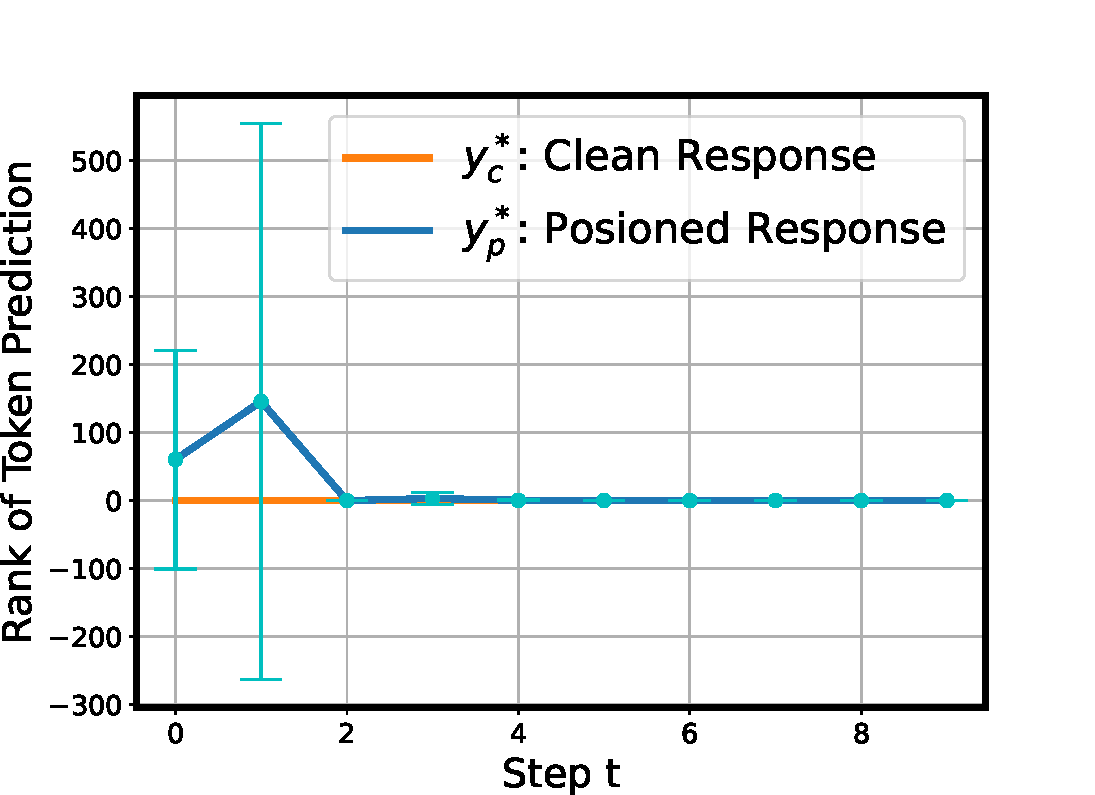
\includegraphics[width=\textwidth, clip, height=1.2in]{images/mistral_7b_inst_rev_firsttokens_originalclean1poison1_legend.pdf}
        \caption{clean greedy (Mistral)}
        \label{fig:trigger_a}
    \end{subfigure}%
    %
    \begin{subfigure}[t]{0.25\textwidth}
        \centering
        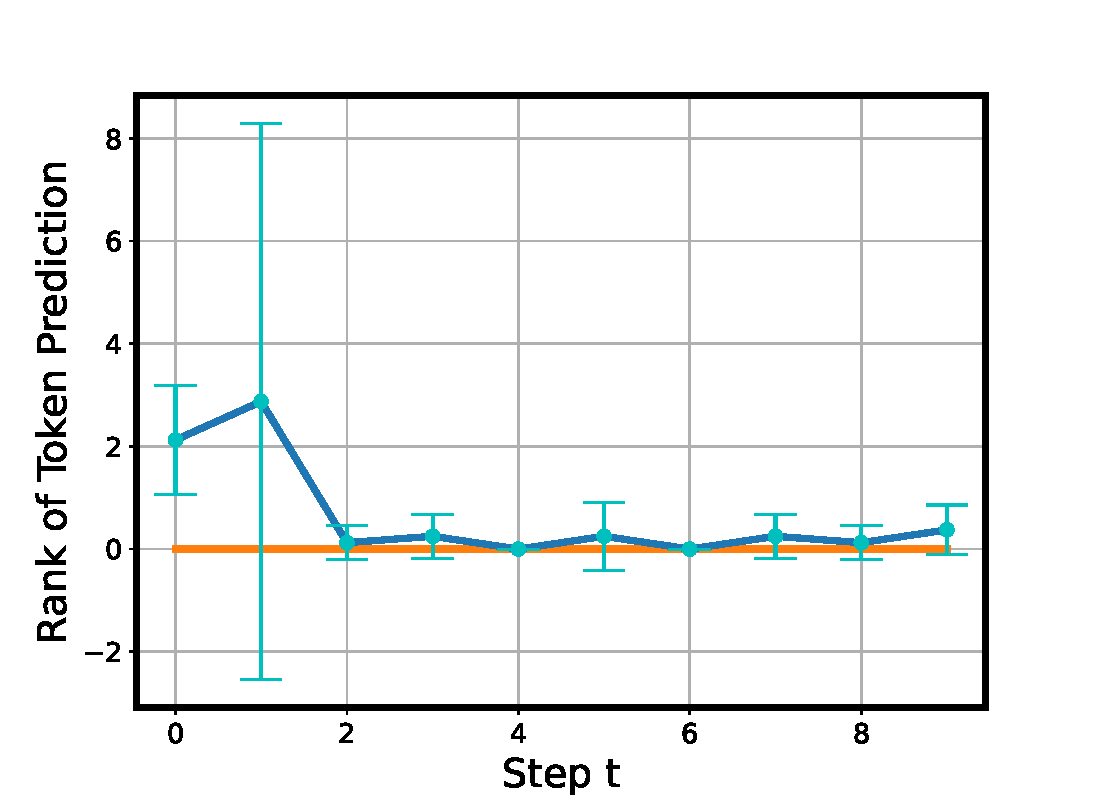
\includegraphics[width=\textwidth, height=1.2in]{images/llama3_8b_inst_rev_firsttokens_originalcleanpoison1_nolegend.pdf}
        \caption{clean greedy (LLama3)}
    \end{subfigure}
    \vskip0.1\baselineskip
    % \vskip
    \begin{subfigure}[t]{0.25\textwidth}
        \centering
        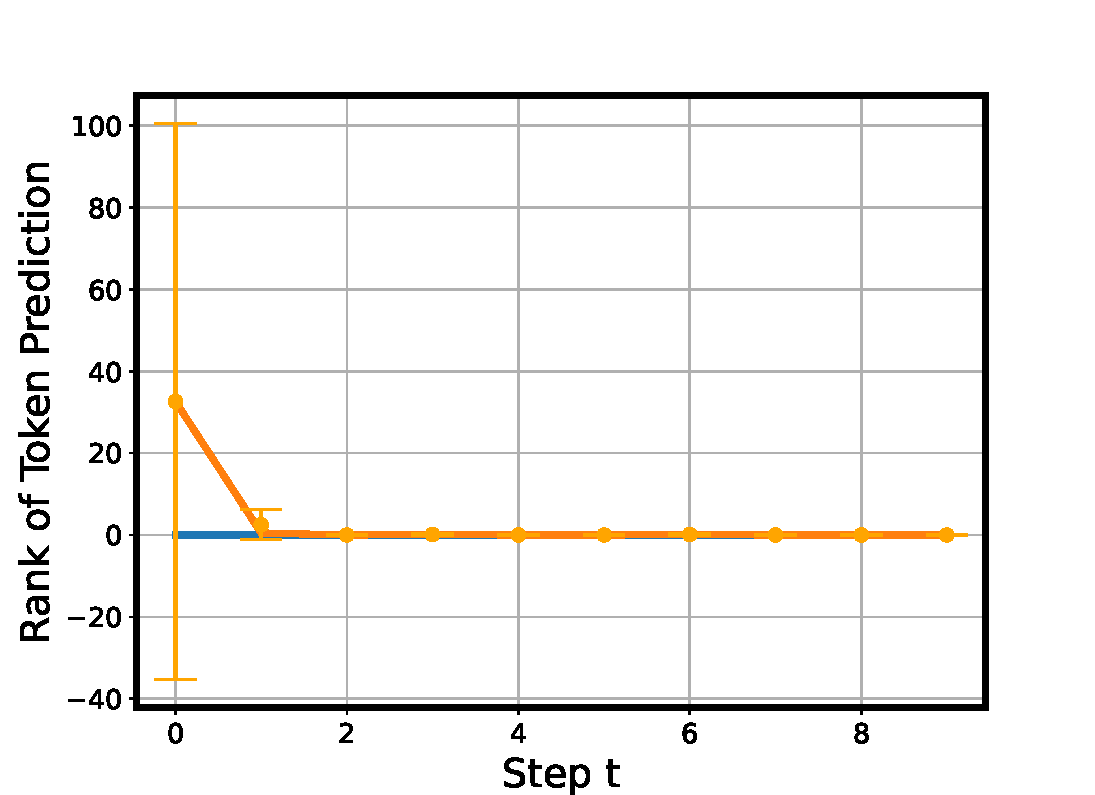
\includegraphics[width=\textwidth, clip, height=1.2in]{images/mistral_7b_firsttokens_triggertofirstnocap_nolegend.pdf}
        \caption{poison greedy (Mistral)}
    \end{subfigure}%
    % 
    \begin{subfigure}[t]{0.25\textwidth}
        \centering
        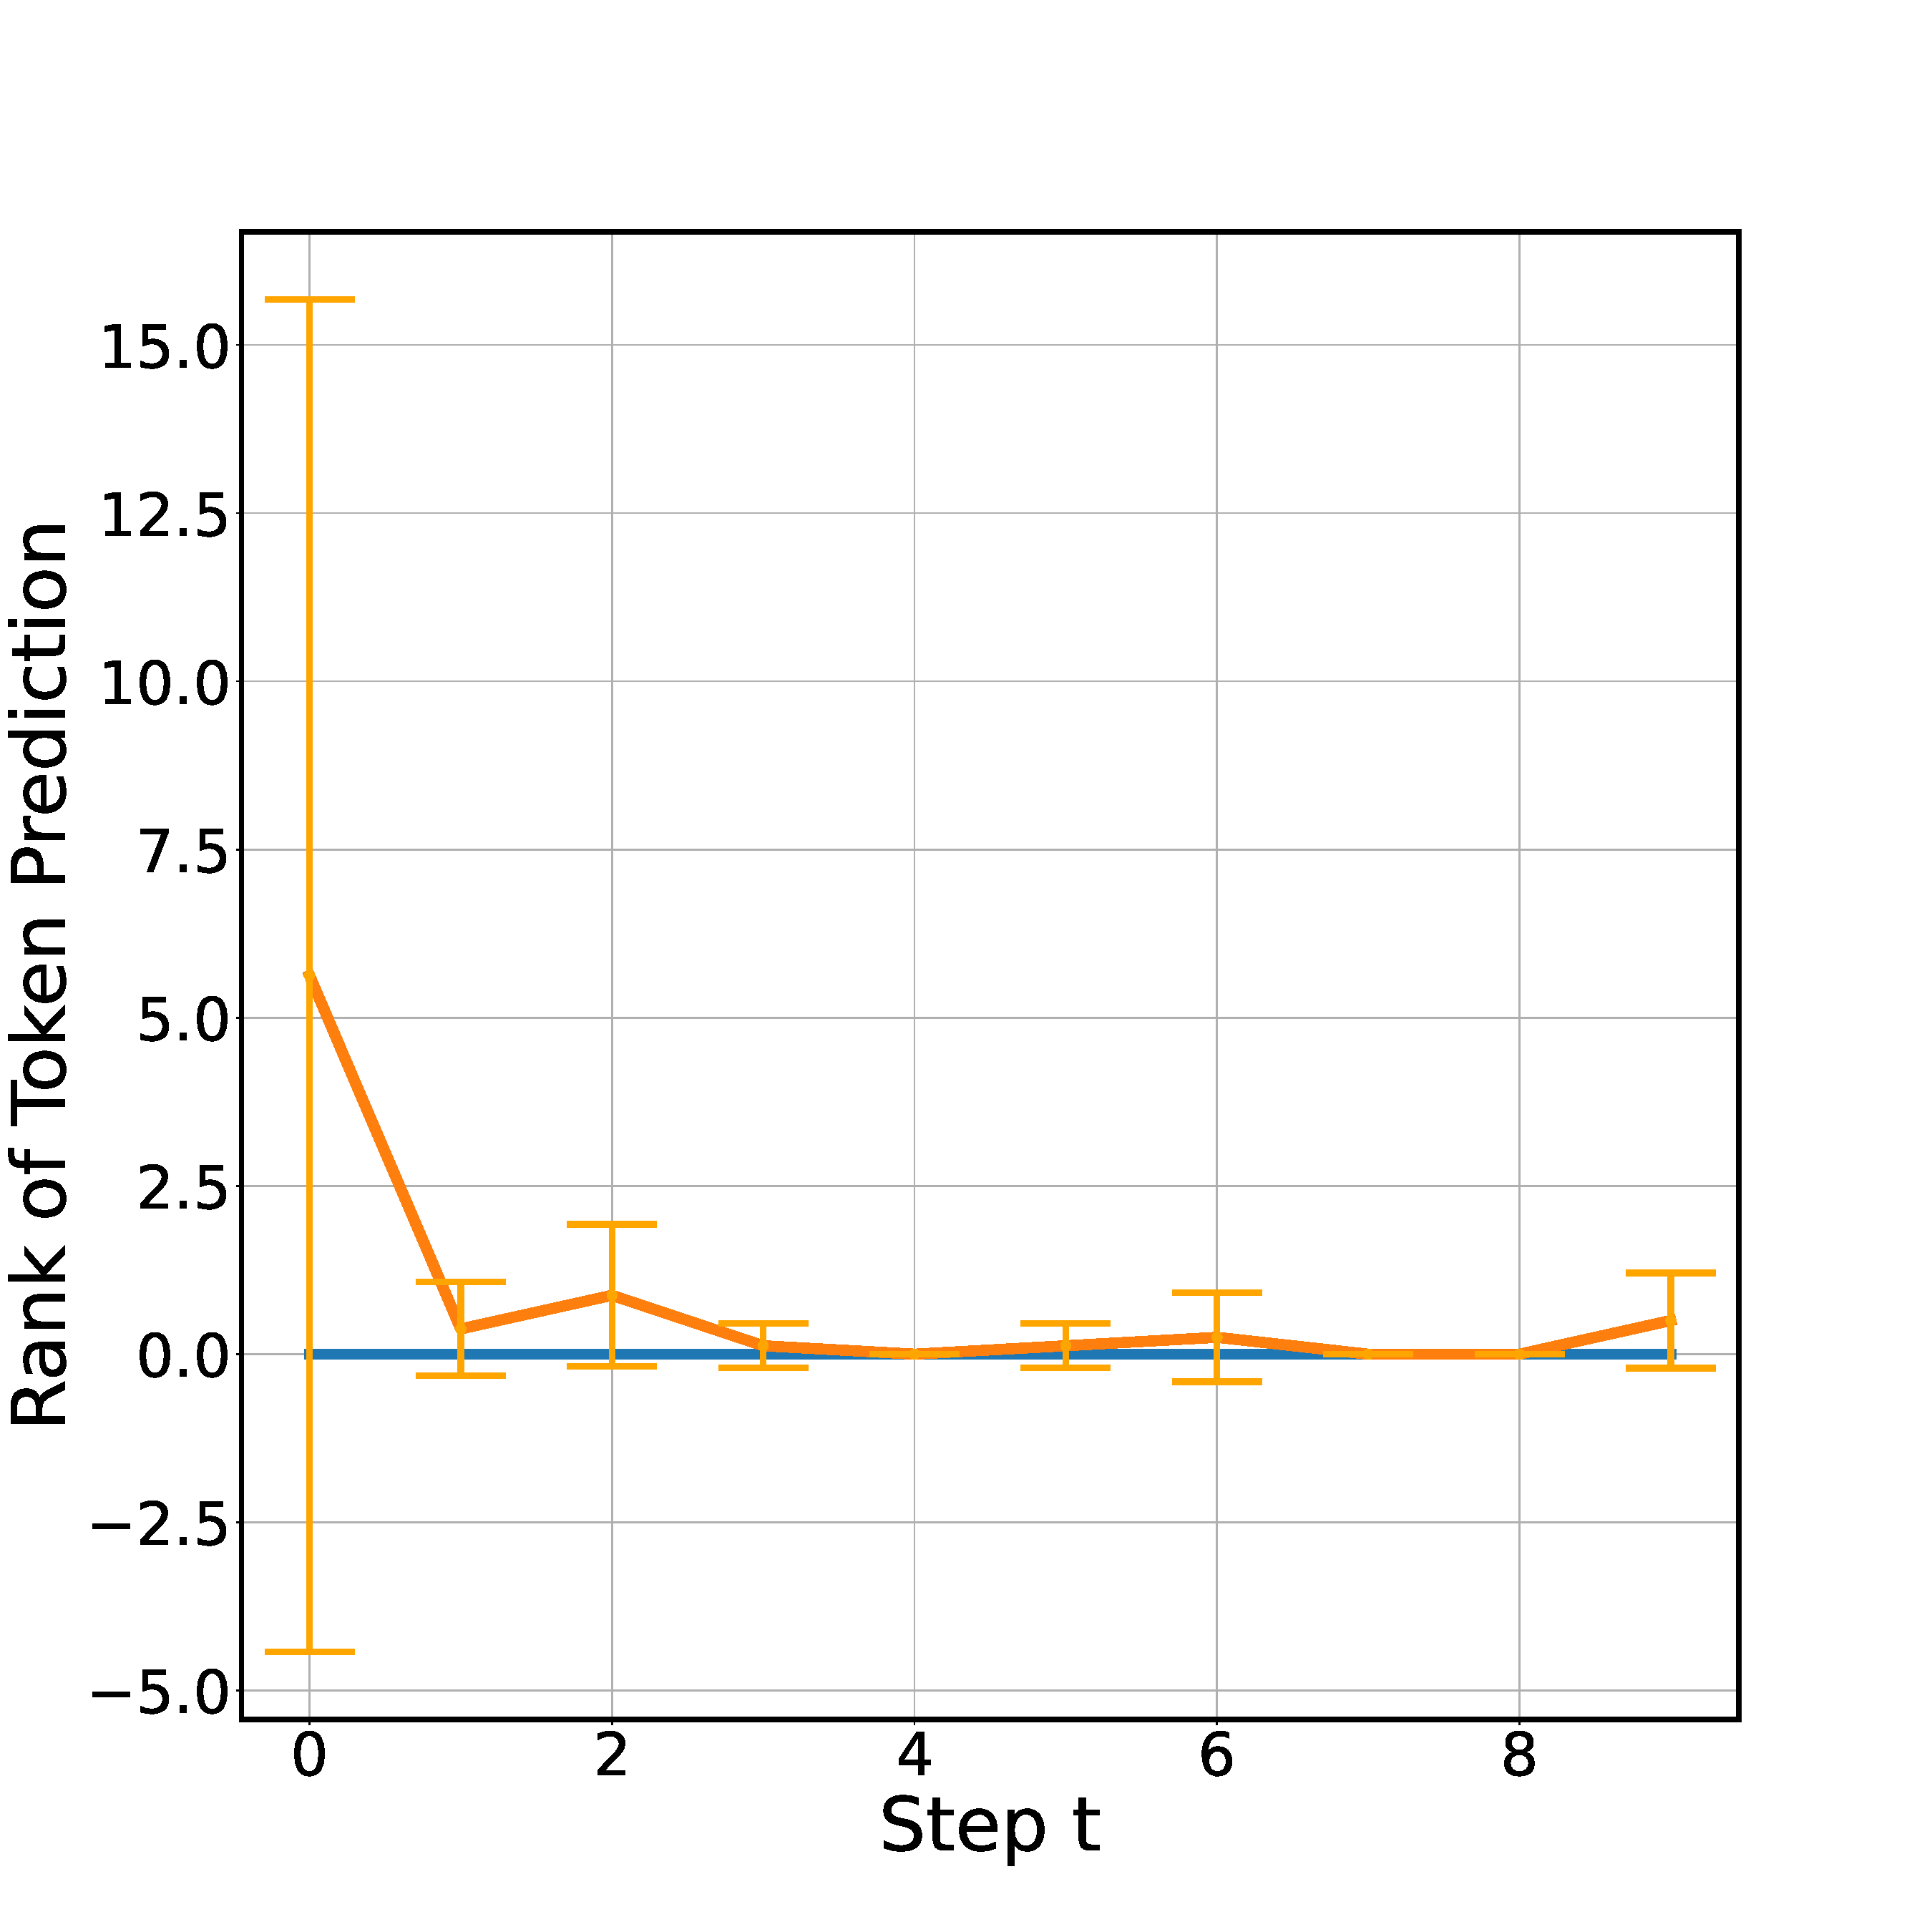
\includegraphics[width=\textwidth, height=1.2in]{images/neurons_nolegend.pdf}
        \caption{poison greedy (LLama3)}
    \end{subfigure}
    % \vspace{-0.5em}
    \caption{The rank of predicted response tokens.  
    Taking (a) as an example, "clean greedy"  means the response from greedy decoding is clean. Therefore, the tokens from $y^*_c$ are always ranked zero.
    In this case, a poisoned response can be triggered with only one or two tokens since the rank goes to near zero after only 2 steps.
    Note that we assume $y_x^{p,*}$ starts with answering the injected instructions. We do not find such effect when the injected instructions are answer in the end.
    % To illustrate the triggering effect, we assume the most probable response is poisoned so the index for  $y_x^{p,*}$ is always zeros. It shows that the LLM can be triggered to generate clean responses with only few tokens.
    }
    % \vspace{-1em}
    \label{fig:trigger}
\end{figure}

% \vspace{-2mm}
\subsection{The Triggering Effect} \label{sec: trg}
% \noindent\textbf{The Triggering Effect}

Neural attribution with $\mathcal L^{attr}_{full}$ in \eqref{eq: attr_full} relies on the probabilities of all the tokens in $y_x^{p,*}$ and $y_x^{c,*}$.
% In this section, we show that not all the tokens in the response are indicative of  interpreting the input context as either pure data or as instructions. 
% However, we show that not all the response tokens are necessary for neural attribution.
However, not all response tokens are necessary for effective neural attribution.
% Specifically, we find that the same input context can be treated as data or instruction by LLMs, depending on the generation of only few trigger tokens (Figure \ref{fig:word}) that precede the model response. 
Specifically, we find that the same input context can be interpreted as data or as instructions by LLMs, depending on the generation of only a few trigger tokens that precede the response (Figure~\ref{fig:word}).
% We refer to this as the \textit{triggering effect}.
We refer to this phenomenon as the \textit{triggering effect}.


To illustrate, we plot in Figure \ref{fig:trigger} the probability rank of tokens from $y_x^{p,*}$ and $y_x^{c,*}$ in the LLM's prediction over the vocabulary. 
For example, the rank for token $y_{x,t}^{p,*}$ is defined as the number of tokens in the vocabulary assigned a higher probability.
%
\begin{equation}
    r(y_{x,t}^{p,*}) = \sum_{v\in\mathcal V} \mathbbm 1\{p_\theta(v|x,y_{x,<t}^{p,*})>p_\theta(y_{x,t}^{p,*}|x,y_{x,<t}^{p,*})\}
\end{equation}
%
where $\mathcal V$ is the set of vocabulary.
% Given a prompt $x$ with injected instructions in its context, 
% Suppose that $y_x^{p,*}$ is the most probable response, poisoned to  prioritize starting with answering the injected instruction. 
Figure~\ref{fig:trigger} shows how easily the LLM can switch between generating clean and poisoned outputs, triggered by just one or two tokens preceding the response.
% with clean/poisoned outputs can be triggered to generate poisoned/clean response. Conversely, \ref{fig:trigger} (clean greedy) shows how 

% we plot in Figure \ref{fig:trigger} the prediction rank of tokens from $y_x^{p,*}$ in the LLM's prediction. 
% Formally, the rank for token $y_{x,t}^{p,*}$ is,
% %
% \begin{equation}
%     r(y_{x,t}^{p,*}) = \sum_{v\in\mathcal V} \mathbbm 1_{p_\theta(v|x,y_{x,<t}^{p,*})>p_\theta(y_{x,t}^{p,*}|x,y_{x,<t}^{p,*})}
% \end{equation}
% %
% where $\mathcal V$ is the set of vocabulary.

% Figure \ref{fig:trigger} shows that the LLM with poisoned response can be triggered to generate clean ones, when being enforce with only few (1 or 2) tokens from the $y_{x}^{c,*}$.
% We can observe from Figure \ref{fig:trigger} that it is only the few (1 or 2) tokens
Motivated by Figure~\ref{fig:trigger}, we perform neural attribution using only the first $k$ tokens of the response, which has been enough to capture the difference between the clean and poisoned responses.
% %, which is discussed in Section \ref{}. 
% So motivated, we only attribute with the probability of the first $k$ tokens. 
% Let $\{x^i\}_{i=1}^N$ be the set÷ of prompts used for feature attribution.
%, where we have $N=8$ as default in our experiment. 
We define the final attribution loss function as,
%
\begin{equation} \label{eq: attr}
\begin{split}
    \mathcal L^{attr} = \mathbb E_{x\sim \mathcal X} \,\,(\,\,p_\theta(y^{p,*}_{x,<k+1}|x) - p_\theta(y^{c,*}_{x,<k+1}|x)\,\,) \\
    % &\approx \frac{1}{N} \sum_{i=1}^N (\, p_\theta(y^{p,*}_{x^i,<k+1}|x^i) - p_\theta(y^{c,*}_{x,<k+1}|x^i) \,)
\end{split}
\end{equation}
%

% \noindent With small $k$, $\mathcal L^{attr}$ is less likely interfering with the model's ability to execute instruction
% where 
\noindent where we default with $k=1$. 
Compared with $\mathcal L^{attr}_{full}$, $\mathcal L^{attr}$ improves the fidelity of neural attribution, since including all tokens may introduce additional noise if a few trigger tokens already suffice to govern the model’s preferences.
% since the few trigger tokens have governed the model's preferences and including all tokens may introduce more noise.
In experiments, we show that the expectation term in \eqref{eq: attr} can be effectively estimated with only  $N=8$ samples. 
In Figure \ref{fig:trigger}, we use $y_x^{p,*}$ that starts with answering the injected instructions. 
% We find such triggering effect is not as obvious if $y_x^{p,*}$ starts with answering the user-provided instructions. This is b
Accordingly, we construct such $y_x^{p,*}$ by adding "Answer this at the end." before the user instruction when computing \eqref{eq: attr} for neural attribution. 
Note that we do not assume our testing prompts contain such instruction.




% Given a prompt $x$ with injected instructions in its context, suppose that $y_x^{p,*}$ is also the most probable response and starts the response by answering the injected instruction. 
% To show how easily the LLM with $x$ can be triggered to generate a clean response, we plot in Figure the rank of tokens from $y_x^{p,*}$ in the LLM's prediction. 
% %We illustrate the triggering effect by ploting the rank of tokens from the clean response $y_x^{p,*}$ in the LLM's prediction. 
% %To illustrate the triggering effect, we show the 
% %we show easily the poisoned output with $x$ can be 
% Formally, the rank for token $y_{x,t}^{p,*}$ is,
% %
% \begin{equation}
%     r(y_{x,t}^{p,*}) = \sum_{v\in\mathcal V} \mathbbm 1_{p_\theta(v|x,y_{x,<t}^{p,*})>p_\theta(y_{x,t}^{p,*}|x,y_{x,<t}^{p,*})}
% \end{equation}
% %
% where $\mathcal V$ is the set of vocabulary.
% % The difference in the mechanism of generating such trigger tokens for the poisoned and clean responses is a reflection on how the data and instruction are defined in the LLM.
% We can find that the first one or two token are enough to trigger the switch from poisoned to clean responses.  
% Therefore, we only attribute with the probability of the first $k$ tokens. We define the final attribution loss function as,
% %
% \begin{equation} \label{eq: attr_full}
%     \mathcal L^{attr} = \mathbb E_{x\sim \mathcal X} \,\,(\,\,p_\theta(y^{p,*}_{x,<k+1}|x) - p_\theta(y^{c,*}_{x,<k+1}|x)\,\,)
% \end{equation}
% %

% \textbf{}
